%        File: main.tex
%     Created: Wed Oct 22 06:00 PM 2008 E
% Last Change: Wed Oct 22 06:00 PM 2008 E
%
\documentclass[a4paper,12pt]{article}

\usepackage{setspace}
\usepackage{cite}
\usepackage{graphicx}
\usepackage{amsmath}
\usepackage{amssymb}
\usepackage{url}

\author{Kefei Lu}
\title{Project II Report:\\Internet Traffic Classification Using Naive Bayesian Analysis}

\doublespacing
\begin{document}
\maketitle
\tableofcontents
\newpage

\section{Introduction}
The internet traffic identification plays an important role in network management. It enables network operators to better predict future network metrics and demands, security personnel to detect network anomalous behaviour, researchers to improve network performance.

% Many traffic analysis researches are based on data mining techniques. For example, T. Auld, et al. proposed a traffic classifier that can achieve high accuracy throughout a range of web application types without any source or destination host address or port information \cite{auld2007bnn}. The supervised machine learning based on Bayesian trained neural network is used in their approach. An advantage of their approach is providing classification without access to the packet contents. This powerful advantage ensures the wide application of the approach in network traffic analysis. 

This project is based on the work of Moore et al \cite{moore2005itc}. They applied a Naive Bayes estimator to categorize traffic by application. Uniquely, their work capitalized on hand-classified network data, using it as input to a supervised Naive Bayes estimator. It was indicated that with the simplest of Naive Bayes estimator they were able to achieve about 65\% accuracy on per-flow classification and with powerful refinements they could improve this value to between than 95\%.

In this project, a simple internet traffic supervised classification system based on the Naive Bayes method \cite{moore2005itc} is implemented using C++ programming language with C standard library and C++ standard template library (STL). 

A complete, full functioning data set system is implemented. The data set system is able to load ARFF files as the WEKA system does. It is able to take as many as $2^{64}-1$ instances, each consists of as many as $2^{64}-1$ attributes. The data set system is able to take numeric attributes and nominal attributes, and is able to be extended to add other attribute types. 

Manipulating on the data set system, the naive Bayes classification (NBC) system is implemented. It is able to test and train on a given data set, with specified parameters as the testing instances, training instances, etc. The classifiers are written in a way that they can be easily extended to other classifiers. For example, the basic classifier class specifies the interface that a classifier should implement, i.e., classifies an instance. Then statistical classifiers implement this interface by using the maximum a posteriori (MAP) criteria. Then the naive Bayes classifier inherits from the statistical classifier by calculating the a posteriori probability assuming that attributes are independent and normally distributed conditioned on a given class. Similarly, the naive Bayes classifier with kernel estimation (NBCKE) inherits from the basic naive Bayes classifier, only having different method to calculate the conditional probability of an attribute. In this way, future classifiers can be easily implemented based on existing ones. In this project, the basic classifier (abstract), statistical classifier (abstract), and the naive Bayes classifier are implemented. The naive Bayes classifier with kernel estimation is left for future implementing.

Additionally, some utility applications are developed to help make preprocessing more efficiently. For example, \verb|grab_inst| grabs all instances lines from an ARFF file, prints them to standard output, throwing out other things. \verb|port_hist| prints the histogram of the port numbers of flows belonging to a certain class in an ARFF file. \verb|reindex| renames the attribute names to increasing integer numbers.

For detailed information, please refer to the project reference manual.

\section{The Algorithms: Naive Bayes Method}
\label{sec:alg}
%\subsection{The Basic Naive Bayes Method}
The naive Bayes classifier uses naive Bayes method in classification. It is based on the criteria that one wishes to choose a class label $i$ for a given instance (observation) $\mathbf{o}=\{a_1,a_2,\ldots,a_M\}$, such that the probability $Pr(c_i|\mathbf{o})$ is maximized. In the above equation, $M$ is the number of attributes that the instance has. This criteria is called Maximum A Posteriori (MAP) criteria. Mathematically, it is written as:
\begin{equation}
    \label{eq:map}
    i = argmax_{i \in \mathbf{I}} {Pr(c_i|\mathbf{o})},
\end{equation}
where $\mathbf{I}$ is the set of all possible values of $i$.

In the sense of naive Bayes method, the a posteriori probability in Eq. \ref{eq:map} can be further written as:
\begin{align}
    Pr(c_i|\mathbf{o}) & = \frac{Pr(\mathbf{o}|c_i)Pr(c_i)}{Pr(\mathbf{o})} \\
    & = \frac{ Pr(c_i) \prod_{k=0}^{M} { Pr(a_k|c_i) } } { \sum_{j=0}^{N} {Pr(c_i) \prod_{k=0}^{M}{Pr(a_k|c_j)} }},
\end{align}
where we assume that the attributes consisting of the observation are independently distributed.

To estimate the conditional probabilities, the naive Bayes method further assumes that random variables $\{A_k|c_j\}$ are normally distributed.

Therefore, it is able to evaluate a posteriori probabilities for all class indices. The classification is made on the class with largest a posteriori probability.

% \subsection{The Naive Bayes Method With Kernel Estimation}
\section{The Project Structure}
\begin{figure}[tbp]
    \centering
    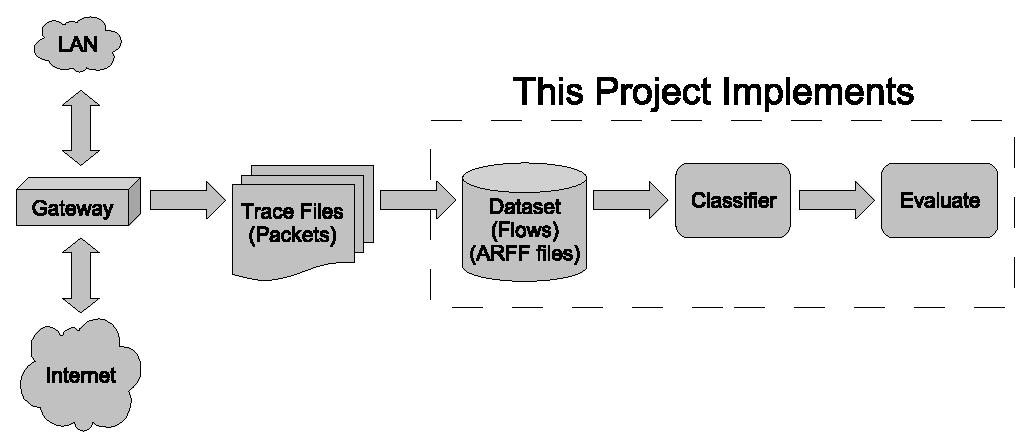
\includegraphics[width=1.1\textwidth]{pic/flow_chart.eps}
    \caption{The flow chart of network traffic classification.}
    \label{fig:flow_chart}
\end{figure} 

As shown in Figure \ref{fig:flow_chart}, the network flow classification process consists of several procedures. A network device records network trace files from the internet. The trace files are then processed during which packet header information are processed and network flows are identified. The flows are recorded in ARFF format to form the desired dataset. The dataset is then feed into the naive Bayes classifier to train the model, then test and evaluate the performance.

It is worth mentioning that it is not trivial to identify flows from packet header traces. Since for this particular project, the authors of \cite{moore2005itc} provides ARFF flow dataset at \cite{moore_website}, I will not focus on the procedure of obtaining traces and identifying flows from packets. For detailed information, please refer to \cite{moore2005duf}.

\section{The Implementation}
Once given the algorithm as described in \ref{sec:alg}, the implementation is straightforward. However, to make the implementation general and extendible is not trivial.

\bibliographystyle{IEEEtran}
% \bibliography{data_mining.bib}{}
\bibliography{data_mining}

\end{document}

